\section{Цепи и антицепи в частично упорядоченных множествах. Теорема Мирского. Теорема Дилуорса.}

$(P, \leq)$ -- ЧУМ

\subsection{Цепи и антицепи в частично упорядоченных множествах}

Цепь в $P$ -- $C \subseteq P: \forall x, y \in C: (x \leq y \lor y \leq x)$

Антицепь в $P$ -- $A \subseteq P: \forall x \neq y \in A: x, y$ -- несравнимы

$|A \cap C| \leq 1$ -- (если как минимум 2 элемента есть, то они не могут быть сравнимы и несравнимы одновременно)

\subsection{Теорема Мирского}
Наименьшее кол-во антицепей, покрывающих ЧУМ равно наибольшей длине цепи в этом ЧУМе

\subsection{Теорема Дилуорса}
Наименьшее кол-во цепей, покрывающих ЧУМ равно наибольшему размеру антицепи в этом ЧУМе

\section{LYM-неравенство, теорема Шпернера о размере максимальной антицепи в булевом кубе.}

Булев куб $\mathbb{B}^n = \{0, 1\}^n$ -- ЧУМ всех подмножеств $\{1,2,\hdots,n\}$ по включению
\[
(a_1, \hdots, a_n) \leq (b_1, \hdots, b_n), \quad 0 < 1
\]
\[
\Updownarrow
\]
\[
\forall i: a_i \leq b_i
\]

Вес $|a|$, $a = (a_1, \hdots, a_n)$ -- колво единиц в $a$

Уровни $\mathbb{B}^n: B_0, B_1, \hdots, B_n$, $B_k = \{a \in \mathbb{B}^n \; | \; |a| = k\}$ 

Макс. размер цепи в $\mathbb{B}^n$ -- $(n+1)$
\vspace{-0.5cm}
{
    \color{gray}
\subsection*{\textit{Доказательство:}}

}

Теорема Шпернера: макс. размер антицепи в $\mathbb{B}^n$ -- $\binom{n}{[n/2]}$

LYM неравенство: Пусть $A$ -- а/ц в $\mathbb{B}^n$, $a_k = |A \cap B_k|$. Тогда:
\[
\sum_{k = 0}^{n} \frac{a_k}{|B_k|} \leq 1
\]

\section{Граф сравнимости частично упорядоченного множества. Совершенные графы. Когда граф является совершенным?}

\subsection{Граф сравнимости частично упорядоченного множества.}

Пусть $(P, \leq)$ -- ЧУМ. Граф сравнимости $P$ -- простой неор. граф $G$:
\[
G = (V, E), V = P: (x, y) \in E \Leftrightarrow \left[
    \begin{matrix}
        \text{$x < y$}\\
        \text{$x > y$}\\
    \end{matrix}
\right.
\]

\subsection{Совершенные графы. Когда граф является совершенным?}

Граф $G$ совершенный, если для любого индуцированного подграфа:
\[
\forall H \subseteq G: \chi(H) = \omega(H)
\]

Граф является совершенным, если он не содержит ни $C_{2k + 1}$, ни $\overline{C_{2k + 1}}$ в качестве индуцированного подграфа при $k > 1$

Граф $G$ совершенный $\Leftrightarrow$ граф $\overline{G}$ совершенный

Для любого конечного ЧУМ $P$ его граф сравнимости $G$:
\begin{center}
    $G$ и $\overline{G}$ -- совершенные
\end{center}


\section{Вероятностное пространство, вероятностное распределение, примеры. Свойства вероятности. Пошаговое задание распределения, дерево событий}

Вероятностное пространство -- $(\underbrace{\Omega}_{\text{эл. исходы}}, \underbrace{P}_{\text{ф-я вероятности}})$

Функция вероятности/вероятностное распределение -- $P: \Omega \rightarrow [0, 1]$:
\[
\begin{cases}
    0 \leq P(\omega_i) \leq 1\\
    \sum_{i = 1}^{n} P(\omega_i) = 1
\end{cases}
\]
Событие $A$ -- подмн-во $A \subseteq \Omega$

Вероятность события $A$ -- $\sum P(\omega_i), \; \omega_i \in A$

Свойства вероятности:
\begin{enumerate}
    \item $P(\emptyset) = 0, P(\Omega) = 1$
    \item $P(A \sqcup B) = P(A) + P(B)$
    \item $P(\overline{A}) = 1 - P(A)$
    \item $A \subseteq B \Rightarrow P(A) \leq P(B)$
\end{enumerate}

Пошаговое задание распределения:

\begin{center}
\begin{tikzpicture}[
    % Настройки размеров (делаем компактно)
    level distance=1.5cm,    % Расстояние по вертикали между уровнями
    sibling distance=2.5cm,  % Расстояние по горизонтали на 1 уровне
    level 2/.style={sibling distance=1.2cm}, % Расстояние на 2 уровне (плотнее)
    % Стиль узлов: кружок, черная граница, белый фон
    every node/.style={circle, draw, inner sep=2pt, minimum size=15pt, font=\footnotesize}
]

    % Корень
    \node {}
        % Левая ветка
        child {
            node {О}
            child {
                node {Р}
                edge from parent node[left, draw=none] {\tiny 0.5}
            }
            child {
                node {О}
                edge from parent node[right, draw=none] {\tiny 0.5}
            }
            edge from parent node[left, draw=none] {\scriptsize 0.5}
        }
        % Правая ветка
        child {
            node {Р}
            child {
                node {Р}
                edge from parent node[left, draw=none] {\tiny 0.5}
            }
            child {
                node {О}
                edge from parent node[right, draw=none] {\tiny 0.5}
            }
            edge from parent node[right, draw=none] {\scriptsize 0.5}
        };

\end{tikzpicture}
\end{center}


Если эксперимент состоит из нескольких шагов, распределение задаётся через дерево событий.

На каждом уровне дерева — возможные исходы текущего шага с условными вероятностями.

Вероятность пути в дереве -- произведение вероятностей вдоль рёбер пути.

Вероятность исхода -- вероятность соответствующего пути от корня до листа.

\section{Формула включений-исключений для вероятностей. Задача о беспорядках.}
\subsection{Формула включений-исключений для вероятностей}
$(\Omega, P): A_1, \hdots, A_n:$
\[
P(A_1 \cup \hdots \cup A_n) = \sum_{k = 1}^{n} (-1)^{k+1} \sum_{1 \leq i_1 < \hdots < i_k \leq n} P(A_{i_1} \cap \hdots \cap A_{i_k})
\]
\subsection{Задача о беспорядках}
Вероятностное пространство $\Omega$, $P = \frac{1}{n!}$ (все равновероятны)

Беспорядок $(p_1, \hdots, p_n)$ -- $\forall i: p_i \neq i$

Пусть $Y_i = \{p \in S_n \; | \; p_i = i\}$ -- $i$-ый элемент на своем месте

$P(\text{$p$ не беспорядок}) \Leftrightarrow \exists i: p \in Y_i \Leftrightarrow P(Y_1 \cup \hdots \cup Y_n)$

$P(Y_1 \cap \hdots \cap Y_k) = \frac{(n-k)!}{n!}$

$P(\text{$\geq 1$ неподвижной точки}) = \sum_{k = 1}^{n} (-1)^{k+1} \binom{n}{k} \cdot \frac{(n-k)!}{n!} = \sum_{k = 1}^{n} \frac{(-1)^{k+1}}{k!}$

\section{Условные вероятности, независимые события. Независимость событий в совокупности, отличие
от попарной независимости событий (приведите явный пример)}

Условная вероятность $P(A|B) = \frac{P(A \cap B)}{P(B)}$, $P(B) > 0$

Условная вероятность -- вероятность $A$ после $B$

События $A$ и $B$ независимые, если $P(A \cap B) = P(A) \cdot P(B)$

Независимость $A_1, \hdots, A_n$ в совокупности:
\[
\forall I \subseteq \{1, \hdots, n\}: P(\bigcap_{i \in I}A_i) = \prod_{i \in I} P(A_i)
\]
Попарная независимость $A_1, \hdots, A_n$:
\[
\forall i \neq j: P(A_i \cap A_j) = P(A_i) \cdot P(A_j)
\]
Попарная независимость не означает независимость в совокупности

Пример:

Подбросим 2 монеты. Пусть событие $A$ -- первая монета О, $B$ -- вторая монета О, $C$ -- монеты выпали одинаковой стороной:

$P(A) = P(B) = P(C) = \frac{1}{2}$

Попарная независимость:
\[
\begin{cases}
    P(A \cap B) = P(A) \cdot P(B) = 1/4, \; \text{ выпало 'ОО'}\\
    P(B \cap C) = P(B) \cdot P(C) = 1/4, \; \text{ 2-ая 'О' $\Rightarrow$ 1-ая 'О'}\\
    P(A \cap C) = P(A) \cdot P(C) = 1/4, \; \text{ 1-ая 'О' $\Rightarrow$ 2-ая 'О'}
\end{cases}
\]
Независимость в совокупности:
\[
P(A \cap B \cap C) =^{?} P(A) \cdot P(B) \cdot P(C)
\]
$P(A \cap B \cap C)$ -- первая и вторая 'О' и они равны

$
P(A \cap B \cap C) = \frac{1}{4}, \text{ выпало 'ОО'}
$

$P(A) \cdot P(B) \cdot P(C) = \frac{1}{2} \cdot \frac{1}{2} \cdot \frac{1}{2} = \frac{1}{8}$
\[
\Downarrow
\]
\[
P(A \cap B \cap C) \neq P(A) \cdot P(B) \cdot P(C)
\]


\section{Формулы Байеса и полной вероятности. Пример с тестом на выявление болезни.}

\subsection{Формула полной вероятности}

Пусть $\Omega = \bigsqcup_{i = 1}^{m} A_i$, $P(A_i) > 0$

Тогда для любого события $B$:
\[
P(B) = \sum_{i = 1}^{m} P(B | A_i) \cdot P(A_i)
\]

Графическая интерпретация:
\begin{center}
    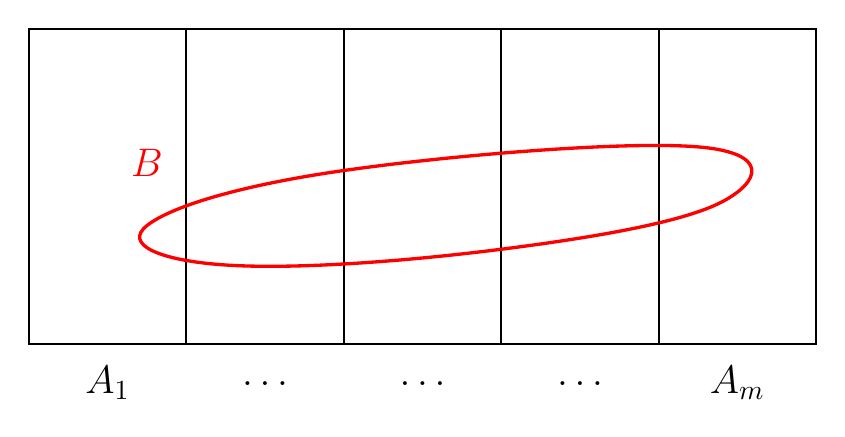
\begin{tikzpicture}[font=\Large]

    % 1. Рисуем черный прямоугольник (пространство Омега)
    % Координаты: (0,0) - левый нижний, (10,4) - правый верхний
    \draw[thick, black] (0,0) rectangle (10,4);

    % 2. Рисуем вертикальные полоски (разбиение A_i)
    \draw[thick] (2.0, 0) -- (2.0, 4);
    \draw[thick] (4.0, 0) -- (4.0, 4);
    \draw[thick] (6.0, 0) -- (6.0, 4);
    \draw[thick] (8.0, 0) -- (8.0, 4);

    % 3. Подписи снизу (A_1 ... A_m)
    \node at (1.0, -0.5) {$A_1$};
    \node at (3.0, -0.5) {$\dots$};
    \node at (5.0, -0.5) {$\dots$};
    \node at (7.0, -0.5) {$\dots$};
    \node at (9.0, -0.5) {$A_m$};

    % 4. Рисуем красный овал (Событие B)
    % plot [smooth cycle] соединяет точки плавной линией
    \draw[red, very thick] plot [smooth cycle, tension=0.7] coordinates {
        (1.5, 1.5)  % Левый край
        (4.0, 2.2)  % Верхняя часть
        (8.5, 2.5)  % Правый край (верх)
        (8.8, 1.8)  % Правый край (низ)
        (6.0, 1.2)  % Нижняя часть
        (2.5, 1.0)  % Нижняя часть слева
    };

    % 5. Подпись B (внутри овала слева, как на рисунке)
    \node[red] at (1.5, 2.3) {$B$};

\end{tikzpicture}
\end{center}

\subsection{Формула Байеса}
Для любых событий $A, B: P(A) > 0, P(B) > 0$:
\[
P(B | A) = \frac{P(A | B) \cdot P(B)}{P(A)}
\]\\
Пример с тестом на выявление болезни:

Предположим, что некоторый тест правильно предсказывает
наличие или отсутствие определенного заболевания с вероятностью
0,95 (если человек действительно болен, то тест
дает положительный результат с вероятностью 0,95 и наоборот)

1\% населения имеет это заболевание.
Предположим, что чел $X$ прошел тестирование и получил
положительный результат. Какова вероятность того, что $X$
действительно болен?

Пусть события $A$ -- $X$ здоров, $\overline{A}$ -- $X$ болен, $B$ -- тест положительный:
\[
P(B | \overline{A}) = 0.95, P(\overline{A}) = 0.01
\]
\[
P(B | A) = 0.05, P(A) = 0.99
\]
По формуле полной вероятности:
\[
P(B) = P(B | A) \cdot P(A) + P(B | \overline{A}) \cdot P(\overline{A}) = 0.059
\]
Тогда ответ (вероятность болезни после теста):
\[
P(\overline{A} | B) = \frac{P(B | \overline{A}) \cdot P(\overline{A})}{P(B)} = \frac{0.95 \cdot 0.01}{0.059} \simeq 0.161
\]
Несмотря на положительный тест, вероятность наличия болезни $16$\%

\section{Случайная величина. Математическое ожидание случайной величины, линейность матожидания.
Дисперсия случайной величины.}

Пусть $(\Omega, P)$ -- вероятностное пространство:

Случайная величина -- функция $f: \Omega \rightarrow \mathbb{R}$
\[
\Omega = \{w_1, \hdots, w_n\}, f(w_i) = a_i \in \mathbb{R}
\]

\subsection{Математическое ожидание случайной величины, линейность матожидания.}

Мат. ожидание $f$ -- $\mathbb{E}(f) = p_1 \cdot f(w_1) + \hdots + p_n \cdot f(w_n) = \sum_{i = 1}^{n} p_i \cdot f(w_i)$

Свойства:
\begin{enumerate}
    \item $f = c \Rightarrow \mathbb{E}(f) = c$, $c$ -- const
    \item $\mathbb{E}(f + g) = \mathbb{E}(f) + \mathbb{E}(g)$ -- линейность{
            \color{gray}
        \subsection*{\textit{Доказательство:}}
        \[
        \mathbb{E}(f+g) = \sum_{i = 1}^{n} p_i(f(w_i) + g(w_i))=
        \]
        \[
        = \sum_{i = 1}^{n} p_i f(w_i) + \sum_{i = 1}^{n} p_i g(w_i)=\mathbb{E}(f) + \mathbb{E}(g)
        \]
    }
    \item $\mathbb{E}(f \cdot c) = c \cdot \mathbb{E}(f)$, $c$ -- const
    \item $A$ -- событие, $I_A(w_i) = \begin{cases}
        1, \text{ $w_i \in A$}\\
        0, \text{ иначе}\\
    \end{cases}$
    \[
    \mathbb{E}(I_A) = \sum_{w \in \Omega} P(w) \cdot I_A(w) = \sum_{w \in A} P(w) = P(A)
    \]
    \item $\mathbb{E}(f) = \sum_{x \in \mathbb{R}} x \cdot P(f = x)$
\end{enumerate}
\text{}\\
Задача о днях рождения

Пусть есть $n = 28$ людей. $\Omega = \{1, \hdots, 365\}^n$ равновероятно

$f$ -- кол-во пар человек, рожденных в один день. $\mathbb{E}(f) = ?$

\[
f = \sum_{i < j} g_{ij},\quad g_{ij} = \begin{cases}
    1, \text{ $i, j$ в один день}\\
    0 \text{ иначе}
\end{cases}
\]

\[
\mathbb{E}(f) = \sum_{i < j} \mathbb{E}(g_{ij}) =
\]
\[
= \sum_{i < j} P(\text{$i$ и $j$ в один день})
\]

$P(\text{$i$ и $j$ в один день}) = \frac{365}{365^2} = \frac{1}{365} \Rightarrow \mathbb{E}(f) = \binom{n}{2} \cdot \frac{1}{365} = \frac{378}{365} > 1$

\subsection{Вероятностный метод}



\subsection{Дисперсия случайной величины.}

Дисперсия $f$ -- $\mathbb{D}(f) = \mathbb{E}((f-\mathbb{E}(f))^2) \geq 0$
\[
\mathbb{D}(f) = \mathbb{E}(f^2) - (\mathbb{E}(f))^2
\]
\vspace{-2cm}
{
\color{gray}
\subsection*{\textit{Доказательство:}}
\[
\mathbb{E}((f-\mathbb{E}(f))^2) = \mathbb{E}(f^2 - 2 \cdot f \cdot \mathbb{E}(f) + (\mathbb{E}(f))^2) =
\]
\[
=\mathbb{E}(f^2) - 2\mathbb{E}(f)\mathbb{E}(f) + \mathbb{E}((\mathbb{E}(f))^2)= 
\]
\[
=\mathbb{E}(f^2) - 2(\mathbb{E}(f))^2 + (\mathbb{E}(f))^2 = \mathbb{E}(f^2) - (\mathbb{E}(f))^2
\]
}

\section{Неравенства Маркова и Чебышёва.}

\subsection{Неравенство Маркова}

Пусть $f$ -- \textbf{неотрицательная} случ. величина, $\alpha > 0$:
\[
P(f \geq \alpha) \leq \frac{\mathbb{E}(f)}{\alpha}
\]
\vspace{-2cm}
{
\color{gray}
\subsection*{\textit{Доказательство:}}
\[
\mathbb{E}(f) = \sum_{x \in \mathbb{R}} x \cdot P(f = x)
\]
\[
\mathbb{E}(f) = \underbrace{\sum_{x < \alpha} x \cdot P(f = x)}_{\geq 0} + \sum_{x \geq \alpha} x \cdot P(f = x)
\]
\[
\Downarrow
\]
\[
\mathbb{E}(f) \geq \sum_{x \geq \alpha} x \cdot P(f = x)
\]
\[
\sum_{x \geq \alpha} x \cdot P(f = x) \geq \sum_{x \geq \alpha} \alpha \cdot P(f = x) = \alpha \cdot P(f \geq \alpha)
\]
\[
\Downarrow
\]
\[
\mathbb{E}(f) \geq \alpha \cdot P(f \geq \alpha)
\]
}

\subsection{Неравенство Чебышёва}

Пусть $f$ -- случ. величина, $\alpha > 0$:
\[
P(|f - \mathbb{E}(f)| \geq \alpha) \leq \frac{\mathbb{D}(f)}{\alpha^2}
\]
\vspace{-2cm}
{
\color{gray}
\subsection*{\textit{Доказательство:}}
Пусть $g = (f - \mathbb{E}(f))^2 \geq 0$:
\[
P(|f - \mathbb{E}(f)| \geq \alpha) = \underbrace{P(g \geq \alpha^2) \leq \frac{\overbrace{\mathbb{E}(g)}^{\mathbb{D}(f)}}{\alpha^2}}_{\text{по Маркову}}
\]
}